\documentclass[12pt]{article}
\usepackage{mathrsfs}
\usepackage{amssymb,amsmath}


\usepackage{tikz}
\usetikzlibrary{arrows,shapes}
\usetikzlibrary{trees}
\usetikzlibrary{matrix,arrows} 				% For commutative diagram
											% http://www.felixl.de/commu.pdf
\usetikzlibrary{positioning}				% For "above of=" commands
\usetikzlibrary{calc,through}				% For coordinates
\usetikzlibrary{decorations.pathreplacing}  % For curly braces
% http://www.math.ucla.edu/~getreuer/tikz.html
\usepackage{pgffor}							% For repeating patterns

\usetikzlibrary{decorations.pathmorphing}	% For Feynman Diagrams
\usetikzlibrary{decorations.markings}

\tikzset{
	% >=stealth', %%  Uncomment for more conventional arrows
    vector/.style={decorate, decoration={snake}, draw},
    provector/.style={decorate, decoration={snake,amplitude=2.5pt}, draw},
    antivector/.style={decorate, decoration={snake,amplitude=-2.5pt}, draw},
    fermion/.style={draw=black, postaction={decorate},
        decoration={markings,mark=at position .55 with {\arrow[draw=black]{>}}}},
    fermionbar/.style={draw=black, postaction={decorate},
        decoration={markings,mark=at position .55 with {\arrow[draw=black]{<}}}},
    fermionnoarrow/.style={draw=black},
    gluon/.style={decorate, draw=black,
        decoration={coil,amplitude=4pt, segment length=5pt}},
    smallgluon/.style={decorate, draw=black,
        decoration={coil,amplitude=2pt, segment length=3pt}},
    scalar/.style={dashed,draw=black, postaction={decorate}},
    scalarbar/.style={dashed,draw=black, postaction={decorate},
        decoration={markings,mark=at position .55 with {\arrow[draw=black]{<}}}},
    scalarnoarrow/.style={dashed,draw=black},
    electron/.style={draw=black, postaction={decorate},
        decoration={markings,mark=at position .55 with {\arrow[draw=black]{>}}}},
    bigvector/.style={decorate, decoration={snake,amplitude=4pt}, draw},
    photon/.style={decorate, decoration={snake,amplitude=4pt, segment length=5pt}, draw=red},
   particle/.style={draw=blue, postaction={decorate}, decoration={markings,mark=at position .5 with {\arrow[draw=blue]{>}}}},
   antiparticle/.style={draw=blue, postaction={decorate}, decoration={markings,mark=at position .5 with {\arrow[draw=blue]{<}}}}
}

%    \DeclareFontFamily{U}{fsy}{}
%      \DeclareFontShape{U}{fsy}{m}{n}{<->s*[.9]psyr}{}
%    \DeclareSymbolFont{ugrf@m}{U}{fsy}{m}{n}
%  \DeclareMathSymbol{\upkappa}{\mathord}{ugrf@m}{`k}


\begin{document}

%$$m\bar{\psi}\psi=m(\bar{e}_{R}e_{L}+\rm{h.c.})=$$


\noindent
$\mathcal{L}=i\bar{\psi}\gamma_{\mu}\partial^{\mu}\psi-m\bar{\psi}\psi$\newline
\newline
$U(1)$ symmetry: $\psi(x)\to \psi^{'}=e^{i\alpha}\psi$, $\alpha\in\mathbb{R}$\newline
\newline
$\mathcal{L}=\mathcal{L}^{'}\quad\Rightarrow\quad\partial_{\mu}j^{\mu}=\partial_{\mu}(-e\bar{\psi}\gamma^{\mu}\psi)=0\quad\Rightarrow\quad Q=\int d^{3}xj^{0}$ conserved


$$ 
\phi = \left(\begin{array}{c}
\phi^{+}\\
\phi^{0}
\end{array}
\right)\to\frac{1}{\sqrt{2}}\left(\begin{array}{c}
0\\
v+H
\end{array}
\right)
$$

$$
g\bar{\psi}^{L}\phi\psi_{R} \to \frac{g}{\sqrt{2}}v\bar{\psi}^{L}\psi_{R} + \frac{g}{\sqrt{2}}H\bar{\psi}^{L}\psi_{R}
$$

$$
|D\phi|^{2}-V(\phi)\to v^{2}e^{2}\mathcal{A}_{\mu}\mathcal{A}^{\mu} +\frac{1}{2}\left[(\partial_{\mu}H)^{2}-m_{H}H^{2}\right] + \mathcal{A}_{\mu}H \,\rm {interactions} 
$$

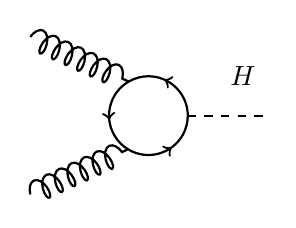
\begin{tikzpicture}[thick,scale=1]
	\draw[gluon] (0,1)--(1.25,0.433);
	\draw[gluon] (0,-1)--(1.23,-0.433);
	\draw[fermion] (2,0) arc (0:120:0.5);
	\draw[fermion] (1.25,0.433) arc (120:240:0.5);
	\draw[fermion] (1.25,-0.433) arc (240:360:0.5);
	\draw[scalar] (2,0)--(3,0);
	\node at (2.7,0.5) {$H$};
\end{tikzpicture} 

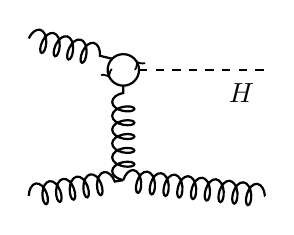
\begin{tikzpicture}[thick,scale=1]
	\draw[gluon] (0,1)--(1.06,0.741);
	\draw[gluon] (0,-1)--(1.2,-0.8);
	\draw[gluon] (1.2,-0.8)--(3,-1);
	\draw[gluon] (1.2,-0.8)--(1.2,0.4);
	\draw[fermion] (1.2,0.4) arc (270:495:0.2);
	\draw[fermion] (1.06,0.741) arc (135:270:0.2);
	\draw[scalar] (1.4,0.6)--(3,0.6);
	\node at (2.7,0.3) {$H$};
\end{tikzpicture} 



\begin{equation}
\vcenter{\hbox{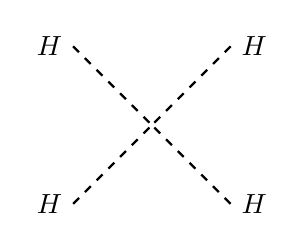
\begin{tikzpicture}[thick,scale=1]
	\draw[scalar](-1,-1)--(0,0);
	\draw[scalar](-1,1)--(0,0);
	\draw[scalar](1,1)--(0,0);
	\draw[scalar](1,-1)--(0,0);	
	\node at (-1.3,-1) {$H$};
	\node at (-1.3,1) {$H$};
	\node at (1.3,1) {$H$};
	\node at (1.3,-1) {$H$};
\end{tikzpicture}}} + \vcenter{\hbox{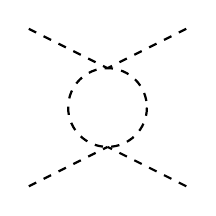
\begin{tikzpicture}[thick,scale=1]
	\draw[scalar](-1,-1)--(0,-0.5);
	\draw[scalar](-1,1)--(0,0.5);
	\draw[scalar](1,1)--(0,0.5);
	\draw[scalar](1,-1)--(0,-0.5);
	\draw[scalar] (0.5,0) arc (360:0:0.5);		
\end{tikzpicture}}} + \vcenter{\hbox{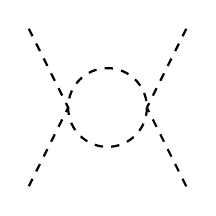
\begin{tikzpicture}[thick,scale=1]
	\draw[scalar](-1,-1)--(-0.5,0);
	\draw[scalar](-1,1)--(-0.5,0);
	\draw[scalar](1,1)--(0.5,0);
	\draw[scalar](1,-1)--(0.5,0);
	\draw[scalar] (0.5,0) arc (360:0:0.5);		
\end{tikzpicture}}}  + \vcenter{\hbox{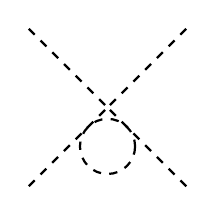
\begin{tikzpicture}[thick,scale=1]
	\draw[scalar](-1,-1)--(0,0);
	\draw[scalar](-1,1)--(0,0);
	\draw[scalar](1,1)--(0,0);
	\draw[scalar](1,-1)--(0,0);	
	\draw[scalar] (0.35,-0.494) arc (360:0:0.35);		
\end{tikzpicture}}} 
\label{eq:lambdaRunning}
\end{equation}

\begin{equation}
\frac{1}{\lambda(v)}-\frac{1}{\lambda(Q)}=\frac{3}{4\pi^{2}}\ln(Q^{2}/v^{2})
\label{eq:triviality}
\end{equation}
\begin{equation}
\lambda(Q) = \frac{\lambda(v)}{1-\frac{3\lambda(v)}{4\pi^{2}}\ln(Q^{2}/v^{2})}
\end{equation}
\begin{equation}
m_{H}^{2} < \frac{8\pi^{2}v^{2}}{3\ln(\Lambda^{2}/v^{2})}
\end{equation}


\begin{equation}
\mathcal{L}_{H} =    
\hbox{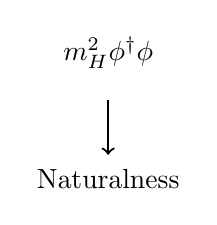
\begin{tikzpicture}[thick,scale=1,baseline=0ex]
	\node at (0,0.1) {$m_{H}^{2}\phi^{\dagger}\phi$};
	\draw [->] (0,-0.5) -- +(0,-0.7);
	\node at (0,-1.5) {Naturalness};
\end{tikzpicture}}
-
\hbox{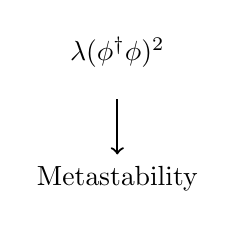
\begin{tikzpicture}[thick,scale=1,baseline=0ex]
	\node at (0,0.1) {$\lambda(\phi^{\dagger}\phi)^{2}$};	
	\draw [->] (0,-0.5) -- +(0,-0.7);
	\node at (0,-1.5) {Metastability};
\end{tikzpicture}}
+
\hbox{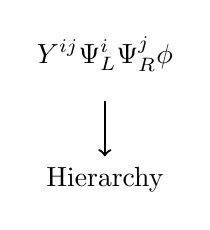
\begin{tikzpicture}[thick,scale=1,baseline=0ex]
	\node at (0,0.1) {$Y^{ij}\Psi^{i}_{L}\Psi^{j}_{R}\phi$};	
	\draw [->] (0,-0.5) -- +(0,-0.7);
	\node at (0,-1.5) {Hierarchy};
\end{tikzpicture}}
\label{eq:HiggsSector}
\end{equation}

\begin{equation}
m_{H}^{2}(\rm{physical})\simeq   
\hbox{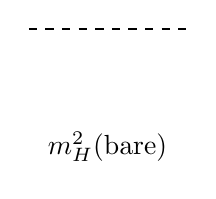
\begin{tikzpicture}[thick,scale=1,baseline=0ex]
	\draw[scalar](-1,0)--(1,0);
	\node at (0,-1.5) {$m_{H}^{2}(\rm{bare})$};
\end{tikzpicture}}
+
\hbox{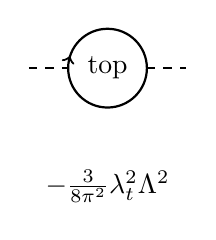
\begin{tikzpicture}[thick,scale=1,baseline=0ex]
	\draw[scalar](-1,0)--(-0.5,0);
	\draw[scalar](0.5,0)--(1,0);
	\draw[fermion] (0.5,0) arc (360:0:0.5);
	\node at (0,0) {top};	
	\node at (0,-1.5) {$-\frac{3}{8\pi^{2}}\lambda_{t}^{2}\Lambda^{2}$};		
\end{tikzpicture}}
+
\hbox{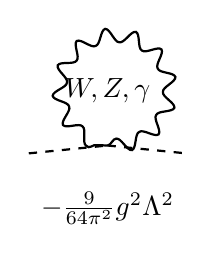
\begin{tikzpicture}[thick,scale=1,baseline=0ex]
	\draw[scalar](-1,-0.8)--(0,-0.7);
	\draw[scalar](0,-0.7)--(1,-0.8);
	\draw[vector] (0,-0.7) arc (-90:270:0.7);
	\node at (0,0) {$W,Z,\gamma$};	
	\node at (0,-1.5) {$-\frac{9}{64\pi^{2}}g^{2}\Lambda^{2}$};		
\end{tikzpicture}}
+
\hbox{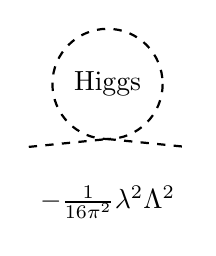
\begin{tikzpicture}[thick,scale=1,baseline=0ex]
	\draw[scalar](-1,-0.8)--(0,-0.7);
	\draw[scalar](0,-0.7)--(1,-0.8);
	\draw[scalar] (0.7,0) arc (360:0:0.7);
	\node at (0,0) {Higgs};	
	\node at (0,-1.5) {$-\frac{1}{16\pi^{2}}\lambda^{2}\Lambda^{2}$};		
\end{tikzpicture}}
\label{eq:HiggsMassCorr}
\end{equation}

\begin{equation}
\delta m_{H}^{2}\,\, \simeq \,\,  
\hbox{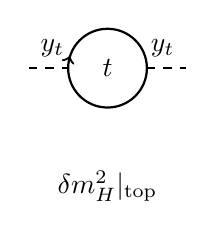
\begin{tikzpicture}[thick,scale=1,baseline=0ex]
	\draw[scalar](-1,0)--(-0.5,0);
	\draw[scalar](0.5,0)--(1,0);
	\draw[fermion] (0.5,0) arc (360:0:0.5);
	\node at (0,0) {$t$};	
	\node at (0,-1.5) {$\delta m_{H}^{2}|_{\rm top}$};
	\node at (-0.7, 0.25) {$y_{t}$};
	\node at (0.7, 0.25) {$y_{t}$};						
\end{tikzpicture}}
+
\hbox{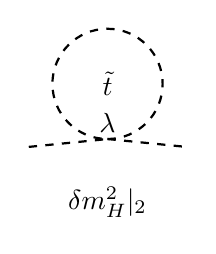
\begin{tikzpicture}[thick,scale=1,baseline=0ex]
	\draw[scalar](-1,-0.8)--(0,-0.7);
	\draw[scalar](0,-0.7)--(1,-0.8);
	\draw[scalar] (0,-0.7) arc (-90:270:0.7);
	\node at (0,0) {$\tilde{t}$};	
	\node at (0,-1.5) {$\delta m_{H}^{2}|_{2}$};
	\node at (0, -0.5) {$\lambda$};		
\end{tikzpicture}}
+
\hbox{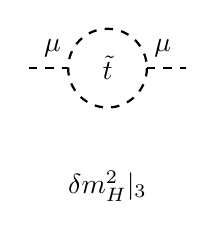
\begin{tikzpicture}[thick,scale=1,baseline=0ex]
	\draw[scalar](-1,0)--(-0.5,0);
	\draw[scalar](0.5,0)--(1,0);
	\draw[scalar] (0.5,0) arc (360:0:0.5);
	\node at (0,0) {$\tilde{t}$};		
	\node at (0,-1.5) {$\delta m_{H}^{2}|_{3}$};
	\node at (-0.7, 0.25) {$\mu$};
	\node at (0.7, 0.25) {$\mu$};			
\end{tikzpicture}}
\label{eq:HiggsMassCorrSUSY}
\end{equation}
\begin{eqnarray}
\delta m_{H}^{2}|_{\rm top} = \frac{N_{C}|y_{t}|^{2}}{8\pi^{2}}\left[  \color{red} -\Lambda^{2} \color{blue} + 3m^{2}_{t}\ln\left(\frac{\Lambda^{2}+m^{2}_{t}}{m^{2}_{t}}\right)\color{black}+...\right]
\label{eq:HiggsMassCorrSUSY1}\\
\delta m_{H}^{2}|_{2} = \frac{\lambda N}{16\pi^{2}}\left[  \color{red} 2\Lambda^{2} \color{blue} - 3m^{2}_{\tilde{t}}\ln\left(\frac{\Lambda^{2}+m^{2}_{\tilde{t}}}{m^{2}_{\tilde{t}}}\right)\color{black}+...\right]
\label{eq:HiggsMassCorrSUSY2}\\
\delta m_{H}^{2}|_{3} = \frac{N}{16\pi^{2}}\left[  \color{blue} - \mu^{2}\ln\left(\frac{\Lambda^{2}+m^{2}_{\tilde{t}}}{m^{2}_{\tilde{t}}}\right)\color{black}+...\right]
\label{eq:HiggsMassCorrSUSY3}\\
\end{eqnarray}


\begin{eqnarray}
\Gamma(H\to f\bar{f}) = N\frac{G_{F}m_{H}m^{2}_{f}}{4\pi\sqrt{2}}\left(1-x_{f}\right)^{3/2}\label{eq:HiggsWidths1}\\
\Gamma(H\to VV) = \frac{G_{F}m^{3}_{H}}{8\pi\sqrt{2}}\sqrt{1-x_{V}}\left(1-x_{V}+\frac{3x_{V}}{4}\right)\left(\frac{1}{2}\right)_{Z}\label{eq:HiggsWidths2}
%\Gamma(H\to WW) = \frac{G_{F}m^{3}_{H}}{8\pi\sqrt{2}}\sqrt{1-x_{W}}\left(1-x_{W}+\frac{3x_{W}}{4}\right)\label{eq:HiggsWidths3}
\end{eqnarray}

$\mathcal{P}_{\rm event}=\mathcal{P}(\Delta\theta_{\rm 3D,1},p_{\tau,1})\times\mathcal{P}(\Delta\theta_{\rm 3D,2},p_{\tau,2})$


\end{document}
